\begin{adjustwidth*}{}{-2.25in}
\textbf{{\large Exercises}}
\setlength{\columnsep}{25pt}
\begin{multicols*}{2}
\noindent Terms and Concepts \small
\begin{enumerate}[1)]
\item In your own words, explain the difference between implicit functions and explicit functions.
\item Implicit differentiation is based on what other differentiation rule?
\end{enumerate} 

\noindent {\normalsize Problems} \small

\noindent {\bf In exercises 3--6, compute the derivative of the given function.}

\begin{enumerate}[1),resume]
\item $\ds f(x) = \sqrt[3]{x}$
\item $\ds f(t) = \sqrt{1-t^2}$
\item $\ds g(t) = \sqrt{t}\sin(t)$
\item $\ds h(x) = x^{1.5}$
\end{enumerate}

\noindent {\bf In exercises 7--17, compute the derivative using implicit differentiation.}

\begin{enumerate}[1),resume]
\item $\ds x^4+y^2+y=7$
\item $\ds x^{2/5}+y^{2/5}=1$
\item $\ds \cos (x)+\sin (y)=1$
\item $\ds \frac{x}{y}=10$
\item $\ds \frac{y}{x}=10$
\item $\ds x^2e^2+2^y=5$
\item $\ds x^2\tan(y)=50$
\item $\ds (3 x^2+2 y^3)^4=2$
\item $\ds (y^2+2y-x)^2=200$
\item $\ds \frac{x^2+y}{x+y^2}=17$
\item $\ds \frac{\sin (x)+y}{\cos (y)+x}=1$
\end{enumerate}

\noindent {\bf In exercises 18--22, find the equation of the tangent line to the graph of the implicitly defined function at the given points.}

\begin{enumerate}[1),resume]
\item $\ds x^{2/5}+y^{2/5} = 1$
\begin{enumerate}
\item	At $(1,0)$.
\item	At $(0.1,0.281)$ (which does not \textit{exactly} lie on the curve, but is very close).
\end{enumerate}
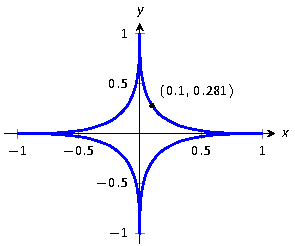
\includegraphics[scale=.8]{figures/fig02_06_ex_23}

\item $\ds x^{4}+y^{4} = 1$
\begin{enumerate}
\item	At $(1,0)$.
\item	At $(\sqrt{0.6},\sqrt{0.8})$.
\item	At $(0,1)$.
\end{enumerate}
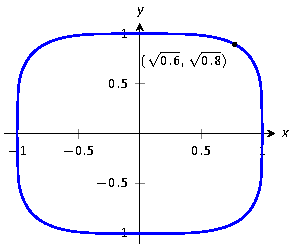
\includegraphics[scale=.8]{figures/fig02_06_ex_24}

\item $\ds (x^2+y^2-4)^3 = 108y^2$
\begin{enumerate}
\item	At $(0,4)$.
\item	At $(2,-\sqrt[4]{108})$.
\end{enumerate}
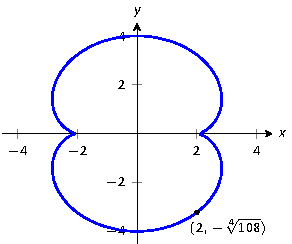
\includegraphics[scale=.8]{figures/fig02_06_ex_25}

\item $\ds (x^2+y^2+x)^2 = x^2+y^2$
\begin{enumerate}
\item	At $(0,1)$.
\item	At $\ds \left(-\frac34, \frac{3 \sqrt{3}}{4}\right)$.
\end{enumerate}
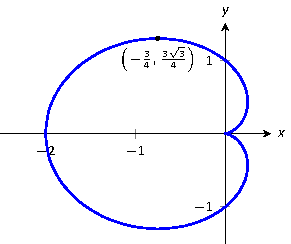
\includegraphics[scale=.8]{figures/fig02_06_ex_26}

\item $\ds (x-2)^2+(y-3)^2=9$
\begin{enumerate}
\item	At $\ds \left(\frac72,\frac{6+3\sqrt{3}}{2}\right)$.
\item	At $\ds\left(\frac{4+3\sqrt{3}}{2}, \frac32\right)$.
\end{enumerate}
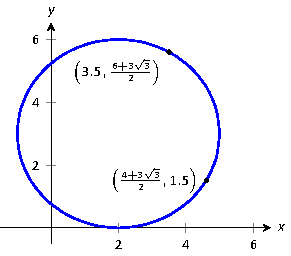
\includegraphics[scale=.8]{figures/fig02_06_ex_27}
\end{enumerate}

%------------------------------------------
% END OF EXERCISES ON FIRST PAGE
%------------------------------------------
\end{multicols*}
\end{adjustwidth*}

\clearpage

\begin{adjustwidth*}{}{-2.25in}
\setlength{\columnsep}{25pt}
\begin{multicols*}{2}\small

\noindent{\bf In exercises 23--26, compute the second derivative of the implicitly defined function.}

\begin{enumerate}[1),start=23]
\item $\ds x^4+y^2+y=7$
\item $\ds x^{2/5}+y^{2/5}=1$
\item $\ds \cos (x)+\sin (y)=1$
\item $\ds \frac{x}{y}=10$

\item Consider the curve given by the equation $2y^3+y^2-y^5 = x^4 - 2x^3  + x^2$.  Find all points at which the tangent line to the curve is horizontal or vertical.

\item For the curve given by the equation $\sin(x+y) + \cos(x-y) = 1$, find the equation of the tangent line to the curve at the point $(\frac{\pi}{2}, \frac{\pi}{2})$.
\end{enumerate}

%---------------------------------------------
% END OF EXERCISES ON SECOND PAGE
%---------------------------------------------
\end{multicols*}
\end{adjustwidth*}

\afterexercises